\documentclass{article}
\usepackage[utf8]{inputenc}

\usepackage{graphicx,caption}
\graphicspath{ {./images/} }
\usepackage{float}
\usepackage{caption}
\usepackage{subcaption}
\usepackage[unicode]{hyperref}
\usepackage{amsmath}
\usepackage[shortlabels]{enumitem}

\title{Homework 4 - Theory/Laboratory}
\author{Dainese Fabio, 857661}
\date{March 29, 2020}

\begin{document}

\maketitle

\section{Reading and Comprehension}
    \begin{enumerate}
        \item The algorithm provided in the \textit{Blondel et al. (2008)} to find the optimal value of \(Q(C)\) can be described by the following two steps:
        \begin{enumerate}
            \item First, each node in the network is assigned to its own community. Then for each node \(i\), the change in modularity is calculated by removing \(i\) from its own community and moving it into the community of each neighbor \(j\) of \(i\).\newline
            Then, once the \(\Delta Q\) value is calculated for all the communities which are directly connected to \(i\), \(i\) is placed into the community that resulted in the greatest modularity increase. If no increase is possible, \(i\) remains in its original community. This process is applied repeatedly and sequentially to all nodes until no modularity increase can occur.
            
            \item In the second phase of the algorithm, it groups all of the nodes in the same community and builds a new network where nodes are the communities from the previous phase. Any links between nodes of the same community are now represented by self-loops on the new community node and links from multiple nodes in the same community to a node in a different community are represented by weighted edges between communities. Once the new network is created and the second phase has ended, the first phase can be re-applied to the new network.
        \end{enumerate}
        
        \noindent The previous steps are iterated until there are no more changes and a maximum of modularity is attained. 
        
        \item The modularity \(Q(C)\) is upper bounded by \(1\) and lower bounded by \(-1\).\newline
        
        \par\noindent To prove that \(Q(C)\) is lower bounded by \(-1\) we have considered the case of having a complete network, which means having the adjacent matrix '\(A\)' equals to all ones except for the diagonal (of zeros - no self-loop allowed in an undirected graph).\newline
        In this scenario we have:
        
        \begin{align*}
            d_{i} &= \sum_{j=1}^{n} = A_{ij} = (n-1) \\
            d &= \frac{1}{2} \sum_{i=1}^{n} \sum_{j=1}^{n} A_{ij} = \frac{(n^{2}-n)}{2} 
        \end{align*}
        
        \noindent Now we are going to use these previous quantities in the modularity formula:
        
        \begin{align*}
            Q(C) &= \frac{1}{2d} \sum_{i=1}^{n}\sum_{j=1}^{n} \left( A_{ij} - \frac{d_{i}d_{j}}{2d} \right) \delta (c_{i},c_{j}) \\
            &= \frac{1}{n^{2}-n} \left[\sum_{i=1}^{n}\sum_{j=1}^{n} \left( A_{ij} - \frac{(n-1)^{2}}{n^{2}-n}\right) \delta (c_{i},c_{j}) \right] \\
            &\leq \frac{1}{n^{2}} \left[\sum_{i=1}^{n}\sum_{j=1}^{n} \left( A_{ij} - \frac{n^{2}}{n^{2}}\right) \delta (c_{i},c_{j}) \right] \\
            &= \frac{1}{n^{2}} \left[\sum_{i=1}^{n}\sum_{j=1}^{n} \left( A_{ij} - 1\right) \delta (c_{i},c_{j}) \right] \\ \intertext{In this particular case of complete graph the value of \(A_{ij}\) will be equals to 1 every time \(i \neq j\), resulting \(( A_{ij} - 1)=(1-1)=0\). The only time in which the multiplication inside the summations is different from zero will be when \(i = j\) \((( A_{ij} - 1)=(0-1)=-1)\) and this happens \(n\) times.\newline Moreover we consider the quantity \(\delta (c_{i},c_{j})\) be equals to \(1\) since we are dealing with an unique giant partition.\newline Then we apply these knowledge into the formula, resulting:}
            &= \frac{1}{n^{2}} \left[n(-1)\right] = - \frac{n}{n^{2}} = - \frac{1}{n}
        \end{align*}
        
        \noindent Finally, we consider the following cases:
        \begin{itemize}
            \item \(n = 1\) : \(Q(C) = - \frac{1}{n} = -1\)
            \item \(n \to \infty\): \(Q(C) = \displaystyle{\lim_{n\to\infty} - \frac{1}{n}} = 0\)
        \end{itemize}
        
        Thus, we have proved that the \(Q(C)\) is lower bounded by \(-1\).\newline\newline
        
        \par\noindent Meanwhile, to prove that \(Q(C)\) is upper bounded by \(1\) we have considered the case of having a network with '\(n\)' isolated \textit{cliques} each of one having \(m\) nodes (meaning that \(|V| = n \cdot m\)). To recall also that the number of edges in a clique of \(m\) nodes is equal to \(\binom{m}{2}\).\newline
        
        \par\noindent As before, we applied these knowledge into the modularity formula, resulting:
        
        \begin{align*}
            Q(C) &= \frac{1}{2d} \sum_{i=1}^{n}\sum_{j=1}^{n} \left( A_{ij} - \frac{d_{i}d_{j}}{2d} \right) \delta (c_{i},c_{j}) \\
            &= \frac{1}{2d} \sum_{k=1}^{n} \left[\binom{m}{2}-\frac{(m-1)^{2}}{2d}\right] \\
            &= \frac{1}{2d} \sum_{k=1}^{n} \left[\frac{m(m-1)}{2}-\frac{(m-1)^{2}}{2d}\right] \\
            &= \frac{1}{2d} \sum_{k=1}^{n} \left[\frac{(m^2-m)d-(m-1)^{2}}{2d}\right] \\
            &= \frac{1}{2d} \sum_{k=1}^{n} \left[\frac{((d-1)m+1)(m-1)}{2d}\right] \\
            &= \frac{((d-1)m+1)(m-1)n}{4d^{2}} \\
            &= \frac{((\frac{nm(m-1)}{2}-1)m+1)(m-1)n}{4\left(\frac{nm(m-1)}{2}\right)^{2}} \\
            &= \frac{((\frac{nm(m-1)}{2}-1)m+1)(m-1)n}{4 \frac{n^{2}m^{2}(m-1)^{2}}{4}} \\
            &= \frac{nm^{2}(m-1)-2m+2}{nm^{2}(m-1)} \\
            &= 1 - \frac{2m-2}{nm^{2}(m-1)} \\
            &= 1 - \frac{2(m-1)}{nm^{2}(m-1)} \\
            &= 1 - \frac{2}{nm^{2}} = 1 - \frac{2}{|V|m}
        \end{align*}
        
        \noindent Finally, if we consider the case of \(|V| \to \infty\), we have:
        \begin{align*}
            Q(C) = \displaystyle{\lim_{|V|\to\infty} \left(1-\frac{2}{|V|m}\right)} = 1 - 0 = 1
        \end{align*}
        Thus, we have proved that the \(Q(C)\) is upper bounded by \(1\).
        
        \item Consider the new partition defined in the given task, we have to prove that:
        \begin{align*}
            Q(\Tilde{C}) - Q(C) &= \frac{k_{2h}}{d} - \frac{k_{1h}}{d} + \frac{d_{h}k_{1}}{2d^{2}} - \frac{d_{h}k_{2}}{2d^{2}} \\
            \intertext{We start by recalling the definition of \(Q(C)\):}
            Q(C) &= \frac{1}{2d} \sum_{i=1}^{n}\sum_{j=1}^{n} \left( A_{ij} - \frac{d_{i}d_{j}}{2d} \right) \delta (c_{i},c_{j})
            = \sum_{i=1}^{R} Q(C_{i})
            \intertext{Where \(Q(C_{i})\) is defined as follows:}
            Q(C_{x}) &= \frac{1}{2d} \sum_{i,j \in C_{x}} \left(A_{ij}-\frac{d_{i}d_{j}}{2d}\right)
        \end{align*}
        \noindent Now we apply these definition to prove the desired result:
        \begin{align*}
            Q(\Tilde{C}) - Q(C) &= \sum_{i=1}^{R} (Q(\Tilde{C_{i}}) - Q(C_{i})) \\
            &= Q(\Tilde{C_{1}}) - Q(C_{1}) + Q(\Tilde{C_{2}}) - Q(C_{2}) + \sum_{i=3}^{R} (Q(\Tilde{C_{i}}) - Q(C_{i})) \\
            \intertext{Since the summation is equals to \(0\), the equation becomes:}
            &= Q(\Tilde{C_{1}}) - Q(C_{1}) + Q(\Tilde{C_{2}}) - Q(C_{2}) \\
            \intertext{Now we substitute the terms with their definitions:}
            \intertext{\[= \frac{1}{2d} \left[ \sum_{i,j \in \Tilde{C_{1}}} \left(A_{ij}-\frac{d_{i}d_{j}}{2d}\right) - \sum_{i,j \in C_{1}} \left(A_{ij}-\frac{d_{i}d_{j}}{2d}\right) + \sum_{i,j \in \Tilde{C_{2}}} \left(A_{ij}-\frac{d_{i}d_{j}}{2d}\right) - \sum_{i,j \in C_{2}} \left(A_{ij}-\frac{d_{i}d_{j}}{2d}\right)\right]\]}
            \intertext{And finally we apply the given definition of \(k_{r}\) and \(k_{rh}\) into the equation, resulting:}
            &= \frac{1}{2d} \left[ 2k_{2h} - 2k_{1h} + \frac{2d_{h}k_{1}}{2d} - \frac{2d_{h}k_{2}}{2d} \right] \\
            &= \frac{k_{2h}}{d} - \frac{k_{1h}}{d} + \frac{d_{h}k_{1}}{2d^{2}} - \frac{d_{h}k_{2}}{2d^{2}}
        \end{align*}
        
        \item Consider the new partition defined in the given task, we have to prove that:
        \begin{align*}
            Q(C) - Q(\Tilde{C}) &=  \frac{d_{h}k_{2}}{2d^{2}} - \frac{k_{2h}}{d}
            \intertext{We start by multiplying all by \(-1\), obtaining:}
            Q(\Tilde{C}) - Q(C) \\
            \intertext{Using the knowledge of the previous point we can substitute the values, resulting:}
            Q(\Tilde{C}) - Q(C) &= \frac{k_{2h}}{d} - \frac{k_{1h}}{d} + \frac{d_{h}k_{1}}{2d^{2}} - \frac{d_{h}k_{2}}{2d^{2}} \\
            \intertext{Since \(\Tilde{C}=\O\) we have that \(k_{1h} = k_{1} = 0\), thus:}
            Q(\Tilde{C}) - Q(C) &= \frac{k_{2h}}{d} - \frac{d_{h}k_{2}}{2d^{2}}
            \intertext{Finally, we multiply all again by \(-1\) and we obtain the expected result, as reported below:}
            Q(C) - Q(\Tilde{C}) &=  \frac{d_{h}k_{2}}{2d^{2}} - \frac{k_{2h}}{d}
        \end{align*}
    \end{enumerate}


\section{Interlocking Directorate}
    \subsection{Subgraph Extraction}
        \begin{figure}[H]
            \centering
            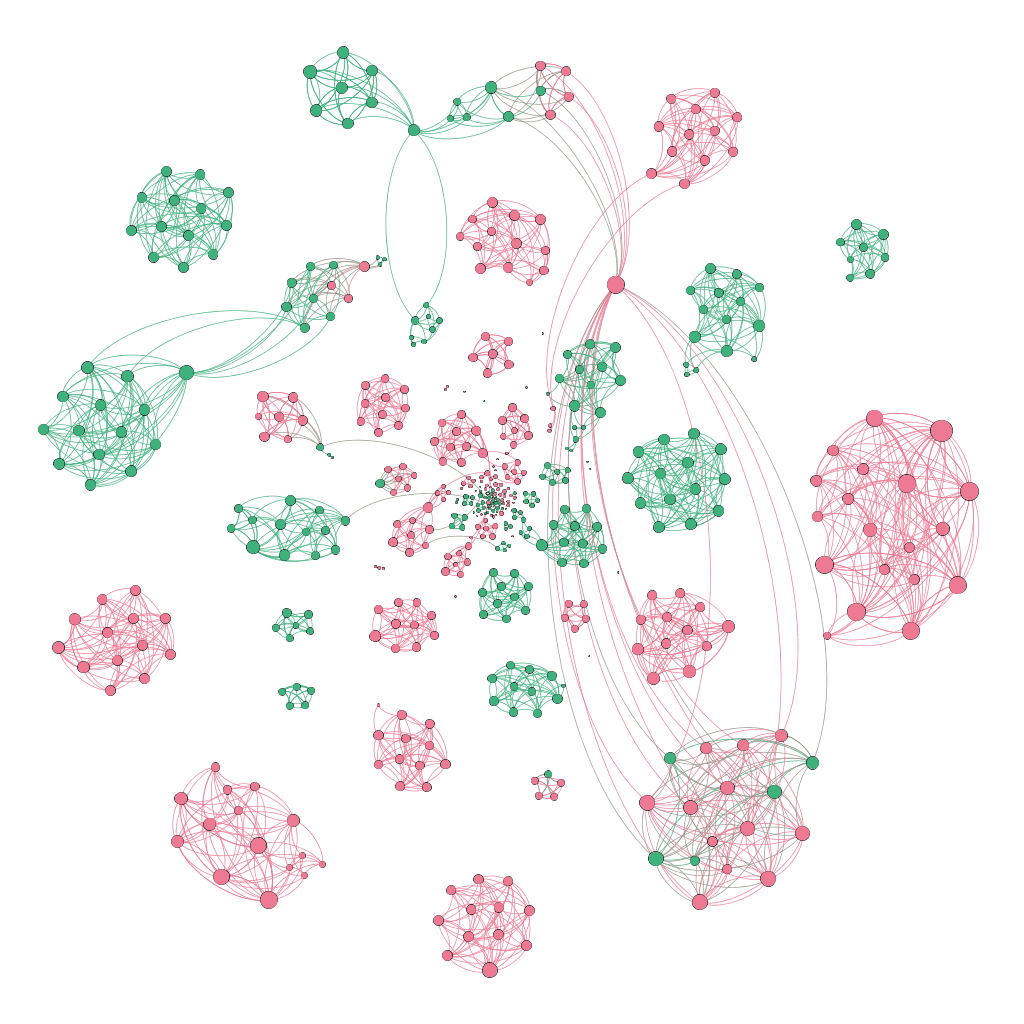
\includegraphics[width=1\textwidth]{1.png}
            \caption{Network}
            \label{fig:figure-1}
        \end{figure}
        
    \subsection{Connected Components}
        In the network represented in 'Figure \ref{fig:figure-1}' there are:
        \begin{itemize}
            \item 533 nodes;
            \item 2251 edges;
            \item 83 weakly connected components.
        \end{itemize}
        
        \noindent Moreover, in the 'Figure \ref{fig:figure-2.0}' are highlighted in red the first and the second largest connected components.
        \begin{figure}[H]
            \centering
            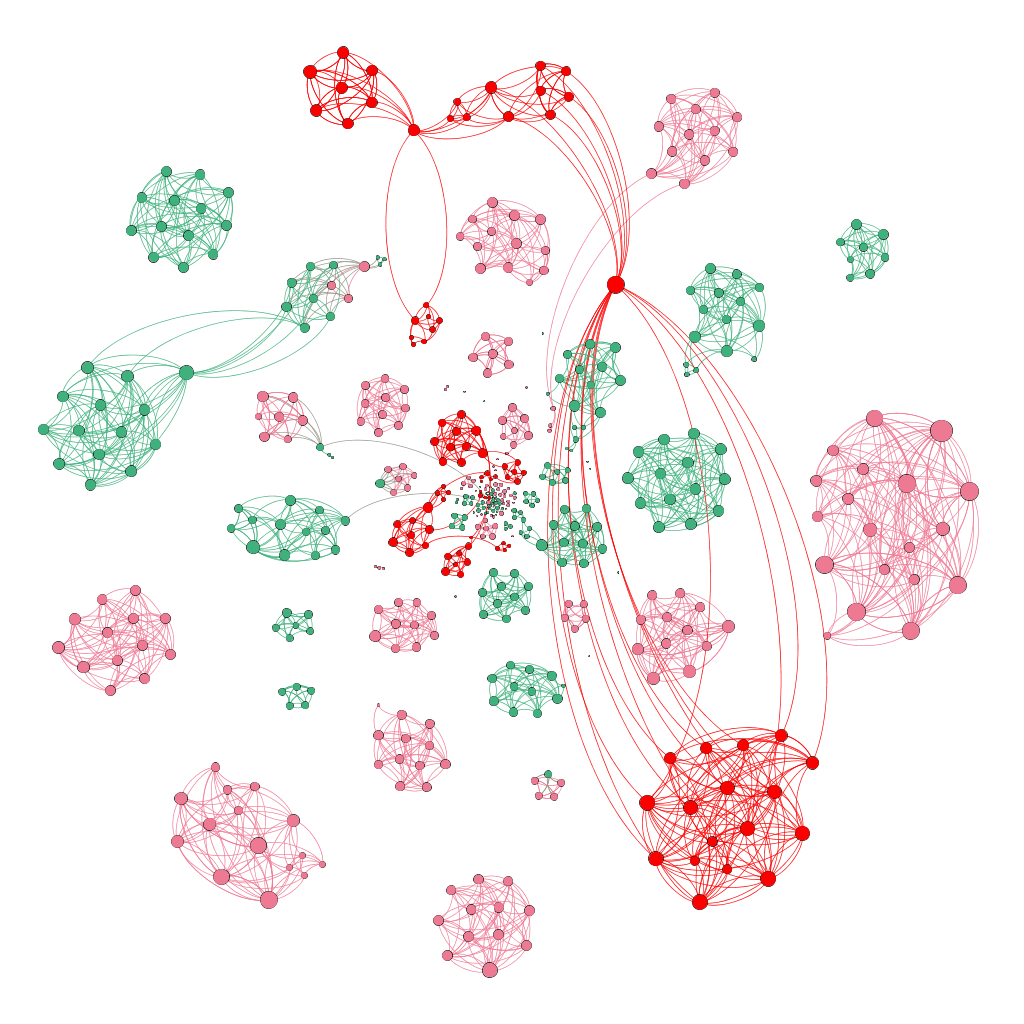
\includegraphics[width=1\textwidth]{2.0.png}
            \caption{}
            \label{fig:figure-2.0}
        \end{figure}
        
        \noindent Just to make it more clear, here the isolated two most largest connected components:
        \begin{figure}[H]
            \centering
            \begin{minipage}[b]{0.4\textwidth}
              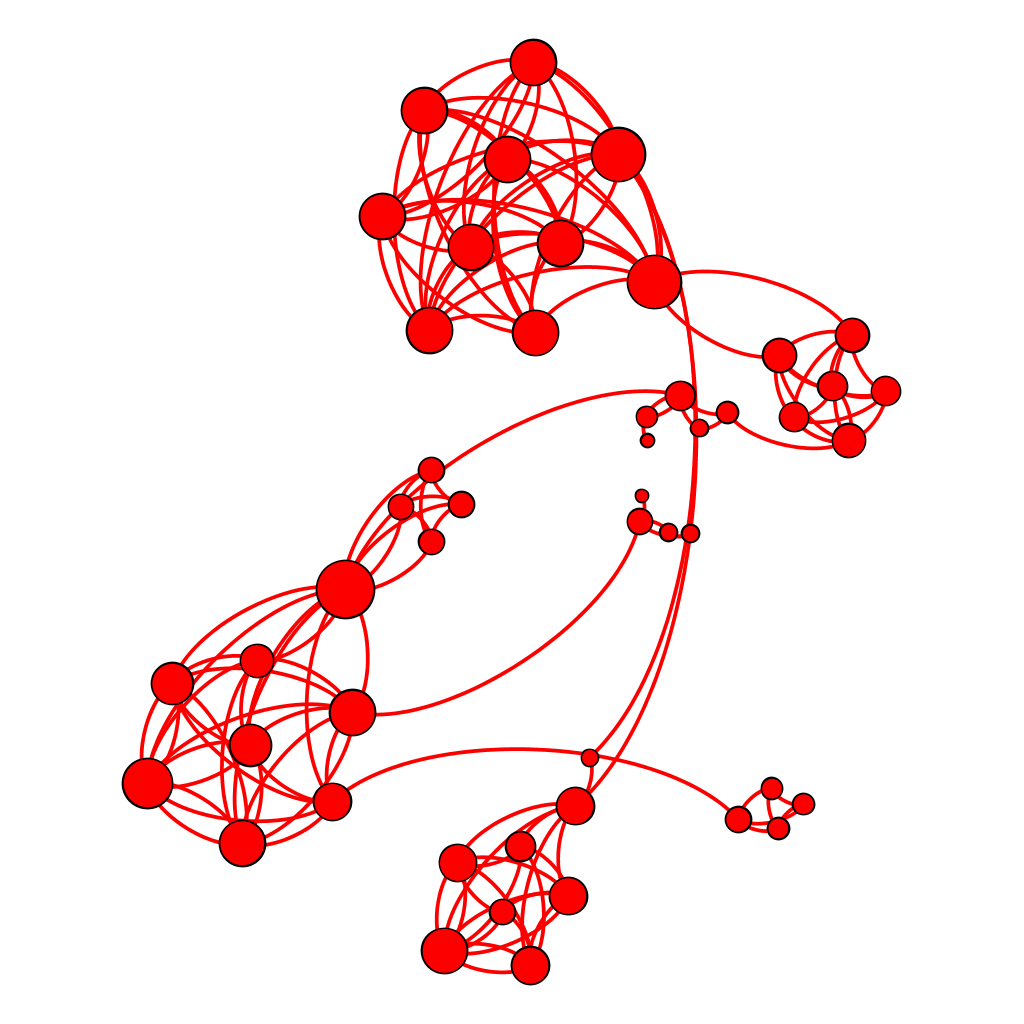
\includegraphics[width=\textwidth]{2.1.png}
                \subcaption{Largest connected component}
            \label{fig:figure-2.1}
            \end{minipage}
            \begin{minipage}[b]{0.55\textwidth}
              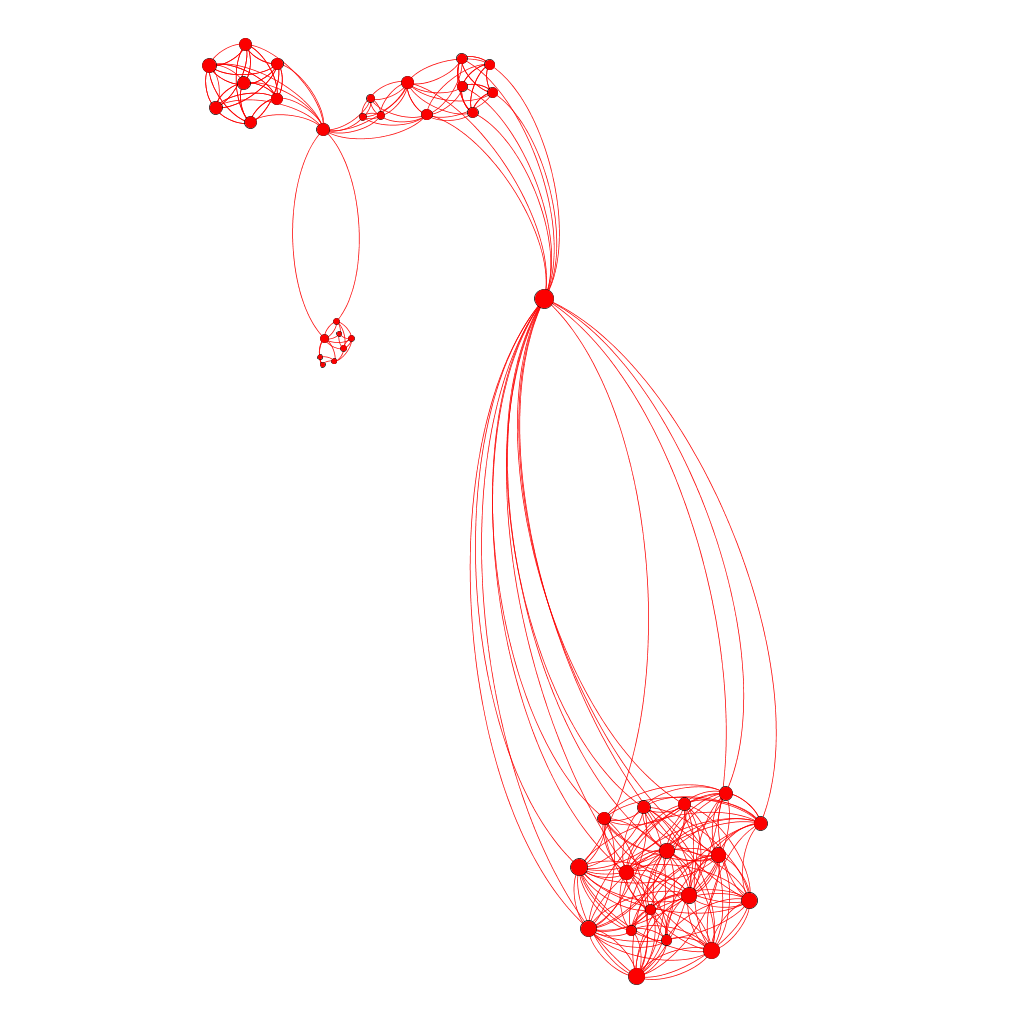
\includegraphics[width=\textwidth]{2.2.png}
                \subcaption{Second largest connected component}
            \label{fig:figure-2.2}
            \end{minipage}
            \label{fig:figure-2}
        \end{figure}
        
        \noindent To isolate the largest connected component it has been used the '\textit{Giant Component}' filter, meanwhile to find the second largest connected component it has been applied the following filters: "Giant Component" \(\to\) "NOT (Nodes)" \(\to\) "Giant Component" (where "\(\to\)" means to applying as a sub-filter).
        
        \subsection{Communities}
        In order to find the communities in the network it has been used the '\textit{Modularity}' statistic  with different resolutions (and without \textit{edge weights}).\newline
        
        \par\noindent With resolution \(0.5\) the results are:
        \begin{itemize}
            \item 89 communities;
            \item 8 communities belonging to the giant component;
            \item By using as a node size the \textit{betweenness centrality} (size between 1 and 16) and colouring each community with a different colour, the result is:
            \begin{figure}[H]
                \centering
             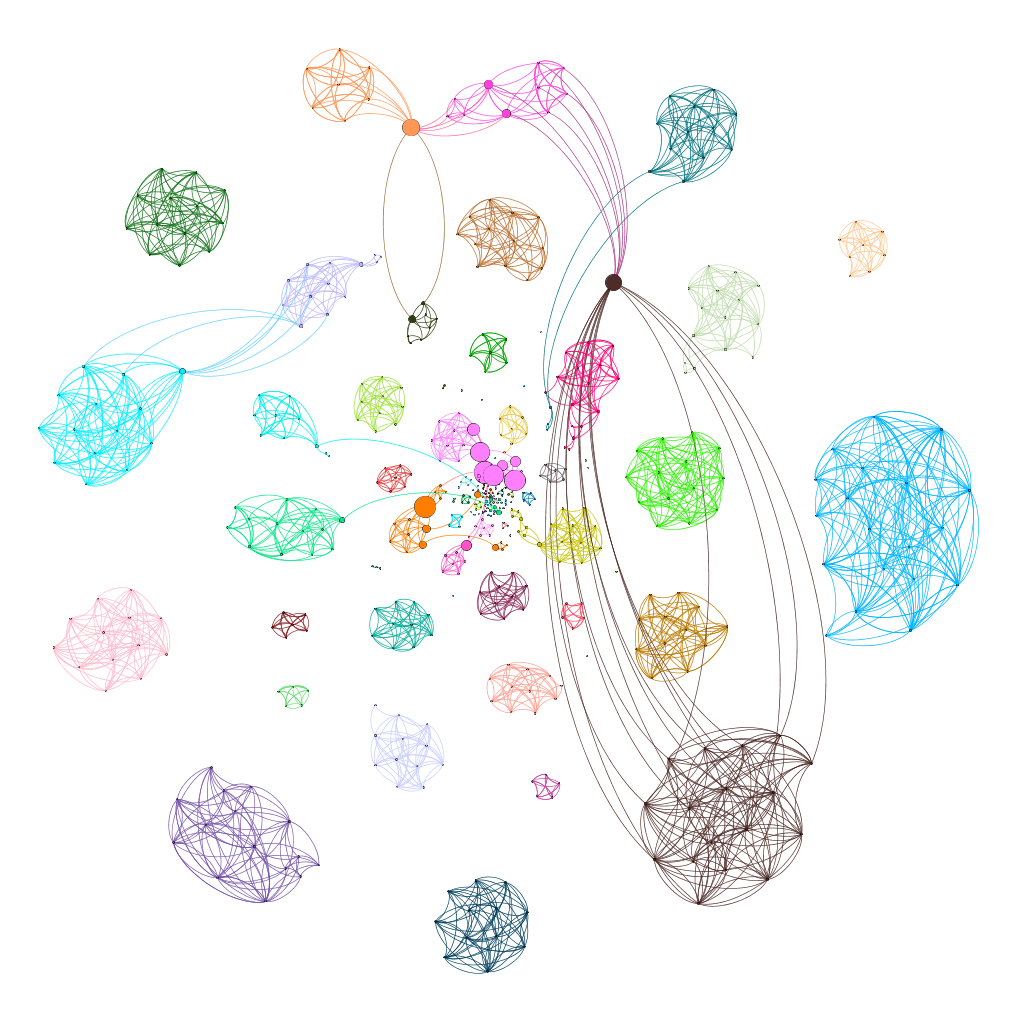
\includegraphics[width=1\textwidth]{3.1.png}
                \caption{}
                \label{fig:figure-3.1}
            \end{figure}
            
        \end{itemize}
        
        \par\noindent Meanwhile with resolution \(1\) the results are:
        \begin{itemize}
            \item 85 communities;
            \item 7 communities belonging to the giant component;
            \item By using as a node size the \textit{betweenness centrality} (size between 1 and 16) and colouring each community with a different colour, the result is:
            \begin{figure}[H]
                \centering
             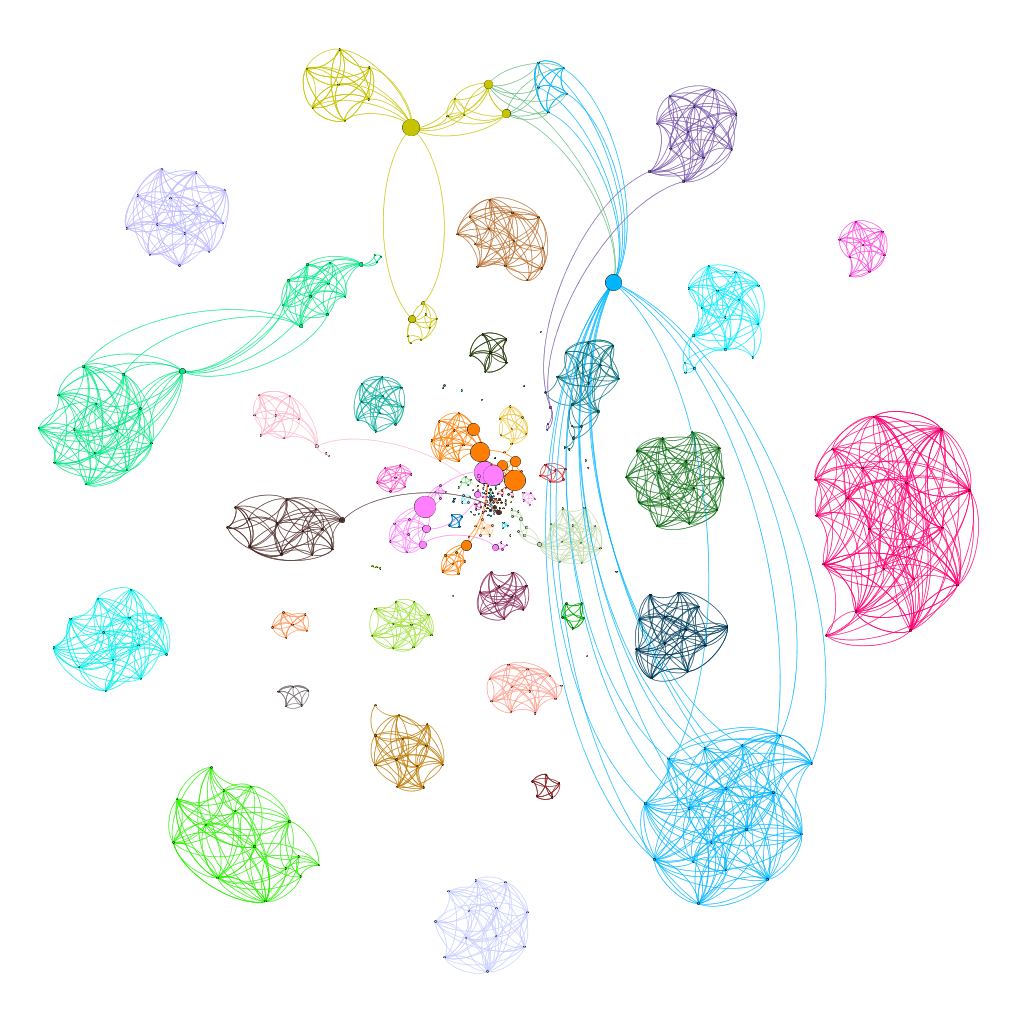
\includegraphics[width=1\textwidth]{3.2.png}
                \caption{}
                \label{fig:figure-3.2}
            \end{figure}
        \end{itemize}
        
        \par\noindent Finally with resolution \(2\) the results are:
        \begin{itemize}
            \item 85 communities;
            \item 6 communities belonging to the giant component;
            \item By using as a node size the \textit{betweenness centrality} (size between 1 and 16) and colouring each community with a different colour, the result is:
            \begin{figure}[H]
                \centering
             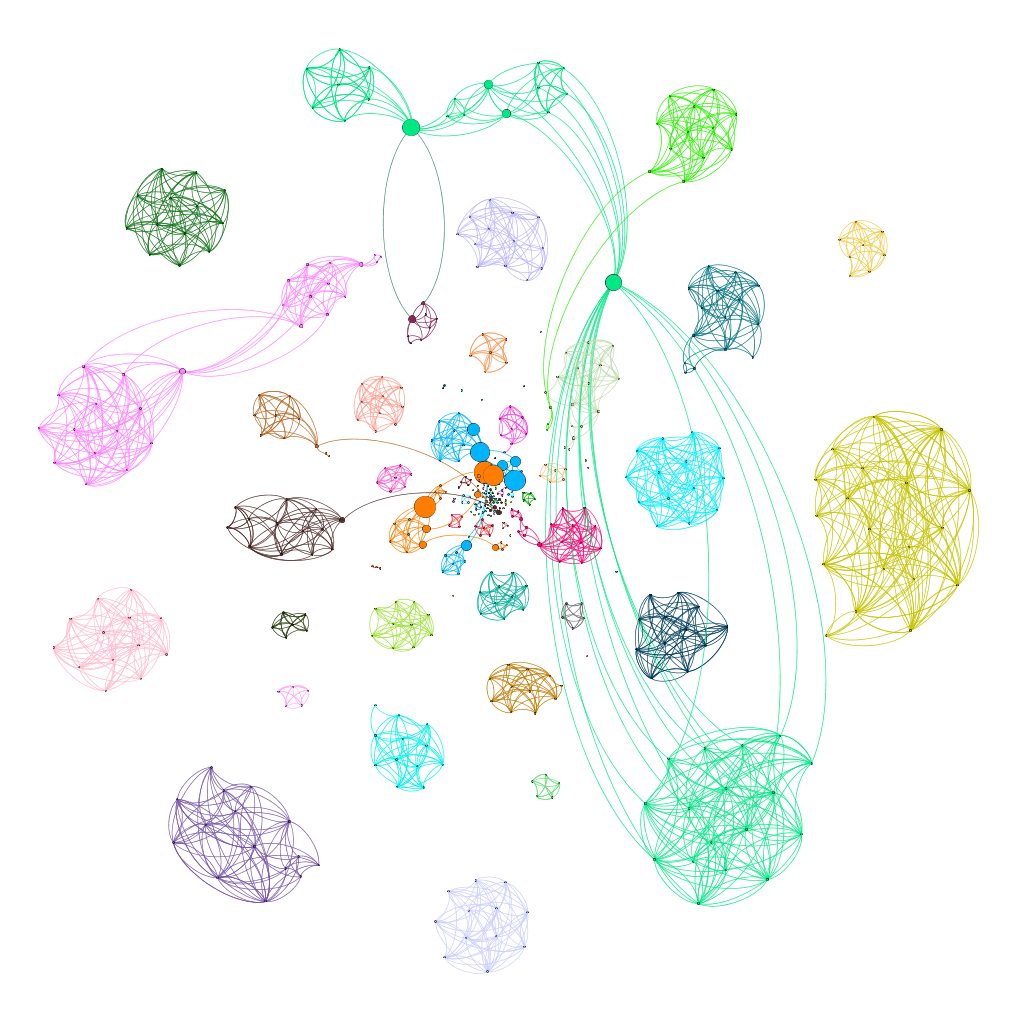
\includegraphics[width=1\textwidth]{3.3.png}
                \caption{}
                \label{fig:figure-3.3}
            \end{figure}
        \end{itemize}
        
        \noindent The number of communities and the number of connected components can be different because the definition of \textit{communities} doesn't imply that there must not be any edges between communities, meanwhile that's a requisite to identify a single connected component.\newline
        
        \par\noindent So, for example, in case of a network composed by a series of isolated cliques, the number of communities and the one of connected components are equal. At the same time if the network is composed by a series of cliques weakly connected between each other, the number of communities and the one of connected components are different.

\end{document}
